% Este documento tem a ver com as partes do LIVRO. 

\thispagestyle{empty}

\begin{textblock*}{-2in}(0pt,0pt)%
\vspace*{-1.8cm}
\hspace*{-3cm}
\includegraphics[width=142mm]{./ABERTURA.png}  
\end{textblock*}

\pagebreak
\blankpage

%\blankpage

% Tamanhos
% \tiny
% \scriptsize
% \footnotesize
% \small 
% \normalsize
% \large 
% \Large 
% \LARGE 
% \huge
% \Huge

% Posicionamento
% \centering 
% \raggedright
% \raggedleft
% \vfill 
% \hfill 
% \vspace{Xcm}   % Colocar * caso esteja no começo de uma página. Ex: \vspace*{...}
% \hspace{Xcm}

% Estilo de página
% \thispagestyle{<<nosso>>}
% \thispagestyle{empty}
% \thispagestyle{plain}  (só número, sem cabeço)
% https://www.overleaf.com/learn/latex/Headers_and_footers

% Compilador que permite usar fonte de sistema: xelatex, lualatex
% Compilador que não permite usar fonte de sistema: latex, pdflatex

% Definindo fontes
% \setmainfont{Times New Roman}  % Todo o texto
% \newfontfamily\avenir{Avenir}  % Contexto
\begingroup\thispagestyle{empty}\vspace*{.05\textheight} 

              \formular
              \huge
              \noindent
              \textbf{Os cantos do\\ homem-sombra}
              
              \vspace{0.3em}

              \noindent\Large\textit{Bat\i{}b’ yám p\I{}n\i{}g}
                    
\endgroup
\vfill
\pagebreak       % [Frontistício]
\newcommand{\linha}[2]{\ifdef{#2}{\linhalayout{#1}{#2}}{}}

\begingroup\tiny
\parindent=0cm
\thispagestyle{empty}

\textbf{edição brasileira\,©}\quad			 {Hedra \the\year}\\
\textbf{narração\,©}\quad						 {Mário Pires e Ponciano Socot}\\
\textbf{organização\,©}\quad					 {Patience Epps e Danilo Paiva Ramos}\\
\textbf{ilustração\,©}\quad	

		 		 {Anita Ekman}\\
\textbf{coordenação da coleção}\quad		 {Luísa Valentini}\\
\textbf{edição}\quad			 			 {Jorge Sallum}\\
\textbf{coedição}\quad			 			 {Suzana Salama}\\
\textbf{assistência editorial}\quad			 {Paulo Henrique Pompermaier}\\
\textbf{capa}\quad			 				 {Lucas Kroëff}\\

\textbf{\textsc{isbn}}\quad			 		 {978-65-89705-73-4} 

\mbox{}\vfill

\begin{minipage}{7cm}
\textbf{Dados Internacionais de Catalogação na Publicação (\textsc{cip})\\
(Câmara Brasileira do Livro, \textsc{sp}, Brasil)}

\textbf{\hrule}\smallskip

Epps, Patience\\

\textit{Os cantos do homem-sombra}. Organização de Patience Epps e Danilo Paiva Ramos.\\ 
2.\,ed. São Paulo, \textsc{sp}: Hedra, 2025.\\

\textsc{isbn} 978-65-89705-73-4\\


1.\,Conto. 2.\,Literatura brasileira. \textsc{i}.\,Epps, Patience. \textsc{ii}.\,Ramos, Danilo Paiva. \textsc{iii}.\,Título.


\hfill \textsc{cdd}: 869.93

\textbf{\hrule}\smallskip

\textbf{Elaborado por Janaina Ramos (\textsc{crb} 8/\,9166)}\\
 

\textbf{Índices para catálogo sistemático:}\\
\textsc{i}.\,Conto: Literatura brasileira

\end{minipage}


\mbox{}\vfill

\textit{Grafia atualizada segundo o Acordo Ortográfico da Língua\\
Portuguesa de 1990, em vigor no Brasil desde 2009.}\\

\textit{Direitos reservados em língua\\ 
portuguesa somente para o Brasil}\\

\textsc{editora hedra ltda.}\\
Rua Sete de Abril, 235, cj.\,102\\
01043--000 São Paulo \textsc{sp} Brasil\\
Telefone/Fax +55 11 3097 8304\\\smallskip
editora@hedra.com.br\\
www.hedra.com.br\\
\bigskip

Foi feito o depósito legal.

\endgroup
\pagebreak
     % [Créditos]
% Tamanhos
% \tiny
% \scriptsize
% \footnotesize
% \small 
% \normalsize
% \large 
% \Large 
% \LARGE 
% \huge
% \Huge

% Posicionamento
% \centering 
% \raggedright
% \raggedleft
% \vfill 
% \hfill 
% \vspace{Xcm}   % Colocar * caso esteja no começo de uma página. Ex: \vspace*{...}
% \hspace{Xcm}

% Estilo de página
% \thispagestyle{<<nosso>>}
% \thispagestyle{empty}
% \thispagestyle{plain}  (só número, sem cabeço)
% https://www.overleaf.com/learn/latex/Headers_and_footers

% Compilador que permite usar fonte de sistema: xelatex, lualatex
% Compilador que não permite usar fonte de sistema: latex, pdflatex

% Definindo fontes
% \setmainfont{Times New Roman}  % Todo o texto
% \newfontfamily\avenir{Avenir}  % Contexto

\begingroup\thispagestyle{empty}\vspace*{.05\textheight} 

              {\formular
              \huge
              \noindent
              \textbf{Os cantos do\\ homem-sombra}

              \vspace{0.3em}
              
              \large
              \noindent
              \textit{Bat\i{}b’ yám p\I{}n\i{}g}
              }              
              \vspace{10em}

              
              {\small\noindent Yuyu-Dëh Mário Pires e Tat-Dëh Ponciano Socot (\textit{narração})}

              {\small\noindent Patience Epps e Danilo Paiva Ramos (\textit{organização})}

              {\small\noindent Anita Ekman (\textit{ilustração})}

              \bigskip

              \noindent
              {\small\noindent 2ª edição}

              \vfill

              \newfontfamily\timesnewroman{Times New Roman}
              {\noindent\fontsize{30}{40}\selectfont \timesnewroman hedra}

              \noindent{\small
              \noindent São Paulo \quad\the\year}


\endgroup
\pagebreak
	       % [folha de rosto]
% nothing			is level -3
% \book				is level -2
% \part				is level -1
% \chapter 			is level 0
% \section 			is level 1
% \subsection 		is level 2
% \subsubsection 	is level 3
% \paragraph 		is level 4
% \subparagraph 	is level 5
\setcounter{secnumdepth}{-2}
\setcounter{tocdepth}{0}

% \renewcommand{\contentsname}{Índex} 	% Trocar nome do sumário para 'Índex'
%\ifodd\thepage\relax\else\blankpage\fi 	% Verifica se página é par e coloca página branca
%\tableofcontents*

\pagebreak
\begingroup \footnotesize \parindent0pt \parskip 5pt \thispagestyle{empty} \vspace*{-0.5\textheight}\mbox{} \vfill
\baselineskip=.92\baselineskip
\textbf{Os cantos do homem-sombra} \lipsum[1]

\textbf{Mário Pires} \lipsum[2]

\textbf{Ponciano Socot} \lipsum[2]

\textbf{Patience Epps} ​é linguista, professora da universidade do Texas em Austin e trabalha com os Hupd’äh desde 2000.

\textbf{Danilo Paiva Ramos} ​é antropólogo, doutor em Antropologia Social pela Universidade de São Paulo, e trabalha com os Hupd’äh desde 2006.

\textbf{Anita Ekman} ​ é ilustradora e atualmente mora na austrália.

\textbf{Coleção Mundo Indígena} reúne materiais produzidos com pensadores de diferentes povos indígenas e pessoas que pesquisam, trabalham ou lutam pela garantia de seus direitos. Os livros foram feitos para serem utilizados pelas comunidades envolvidas na sua produção, e por isso uma parte significativa das obras é bilíngue. Esperamos divulgar a imensa diversidade linguística dos povos indígenas no Brasil, que compreende mais de 150 línguas pertencentes a mais de trinta famílias linguísticas.




\endgroup

\pagebreak\thispagestyle{empty}\movetooddpage
{\begingroup\mbox{}\pagestyle{empty}
\pagestyle{empty} 
% \renewcommand{\contentsname}{Índex} 	% Trocar nome do sumário para 'Índex'
%\ifodd\thepage\relax\else\blankpage\fi 	% Verifica se página é par e coloca página branca
\addtocontents{toc}{\protect\thispagestyle{empty}}
\tableofcontents*\clearpage\endgroup}

\chapter{Introdução}

Os Hupd’äh são um povo indígena que vive em aldeias espalhadas pela floresta Amazônica na região do Alto Rio Negro, no estado do Amazonas, na fronteira com a Colômbia.

A população total é cerca de 1500 pessoas, que moram em 35 aldeias diferentes. Antigamente, moravam de 15 a 50 pessoas nas aldeias Hupd’äh, mas atualmente as comunidades estão maiores e podem abrigar até 200 pessoas.

Os Hupd’äh costumam caçar com arco e flecha e com zarabatana. Pescam diferentes tipos de peixes nos igarapés.­ riachos que corremno interior da mata.

As mulheres dedicam-se diariamente às roças de maniva, um tipo de mandioca, mas também ajudam os homens na caça, na pesca e na coleta de frutas.

Quando viajam para visitar parentes em outras aldeias, os Hupd’äh andam por longos caminhos e acampam à beira do igarapés para descansar. Nestas viagens, é comum que, além de encontrarem animais como pacas, tamanduás, antas e cobras, os Hupd’äh encontrem outros tipos de gente, como a gente­-sombra, gente-­onça e a gente-árvore. Por isso, é preciso ter cuidado e respeitar essas outras gentes, para que elas não façam mal aos viajantes.

A língua hup é a primeira a ser falada pelas crianças Hupd’äh. Esta é uma língua tonal, muito
diferente do português. A língua hup é semelhante às línguas dos povos Yuhupdëh,
Dâw e Nadëb (Kuyawi) que também vivem em comunidades na região do Alto Rio Negro.

Desde 2001, os professores Hupd’äh começaram a participar de cursos para melhorar as
escolas de suas aldeiras. Nesses cursos, os professores Hupd’äh tiveram a ajuda de linguistas e antropólogos para descrever sua língua, criar um modo de escrevê-­la e compreender os princípios gramaticais.

Escutar as histórias dos anciões, gravá­-las, escrevê-­las e reproduzi-­las permite que
crianças e adultos aprendam a ler e escrever na língua Hupd’äh.

Também durante este período, foi elaborado um dicionário Hupd’äh/português, em parceria
com pesquisadores de diferentes Universidades, além de cartilhas da língua hup.
\chapter{Como foi feito este livro}

Em 2002, a linguista Patience Epps morou com os Hupd’äh da aldeia de Barreira Alta para fazer uma pesquisa sobre a língua Hup. Um dia, ela pediu para o senhor Mario Andrade Pires, um sábio ancião hup, contar para ela a história dos \textit{cantos do homem-sombra}.

Patience ouviu atentamente a história, gravou-a com seu gravador, escreveu em seu caderno e depois, com a ajuda dos professores hupd’äh, traduziu a narrativa para o português. Ela pediu também para outras pessoas contarem histórias antigas dos Hupd’äh.

Com estas narrativas ela preparou o livro \textit{Hupd’äh nɨh Pɨnɨ̗gd’äh}, ou os \textit{Contos dos Hupd’äh}, que até hoje ajuda os alunos das escolas Hupd’äh a aprenderem a ler e a escrever em sua língua.

A Hedra interessou-se em publicar essas histórias, numa edição bilíngue. O livro \textit{Batɨ̗b  Yám Pɨnɨ̗g}, \textit{Os cantos do homem-sombra}, traz a primeira história desse livro maior de contos Hupd’äh, enriquecida pelas belas ilustrações de Anita Ekman. Para preparar o livro, Patience contou com a ajuda do antropólogo Danilo Paiva Ramos, que também morou com os Hupd’äh para fazer sua pesquisa.

O canto \textit{Way Naku}, do homem-sombra, que também fez parte desse livro, foi cantado
para o Danilo pelo senhor Ponciano Salustiano Ramos, da aldeia de Tat Dëh, em 2010.



\chapter{Para ler as palavras hup}

Para a grafia em geral dos termos da língua hup, adotou"-se como
referência o dicionário de língua hup elaborado pelo linguista Henri
Ramirez, \textit{A língua dos Hupd'äh do Alto Rio Negro} (Associação Saúde
Sem Limites, 2006). Seguindo Ramirez, mantém-se a acentuação
das vogais de acordo com a nasalidade --- indicada por um \textit{til} --- e o tom --- indicado por um acento grave agudo ou grave.

\section{o alfabeto}

Ramirez propõe que o alfabeto hup tem 25 letras: \textit{a}, \textit{ä}, \textit{b}, \textit{ç}, \textit{e}, \textit{ë}, \textit{g},
\textit{h}, \textit{i}, \textit{ɨ}, \textit{j}, \textit{k}, \textit{m}, \textit{n}, \textit{o}, \textit{ö}, \textit{p}, \textit{r}, \textit{s}, \textit{t}, \textit{u}, \textit{w}, y e '.\footnote{Oclusão
glotal.} Destas, 16 são consoantes, nove são vogais e 11 são consoantes
laringalizadas: \textit{b'}, \textit{d'}, \textit{r'}, \textit{j'}, \textit{g'}, \textit{m'}, \textit{n'}, \textit{w'}, \textit{y'}, \textit{s'}, \textit{k'}.


\part{Os cantos do homem-sombra}

\openany

{\pagecolor{black}
\color{white}
\chapter*{Um canto do homem-sombra}

\letra{O}{utro} galho de cucura\\
Outro galho de cucura\\
Eu jogo para baixo

\bigskip

\noindent Outro galho de cucura\\
Eu jogo para baixo\\
Colho o cacho de cucura\\
Eu jogo para baixo

\bigskip

\noindent \textit{Way Naku, yari nóóy mah\\
Marika, Way Naku}

\chapter*{Way Naku}

\letra{S}{ã̗p} nowot pɨ̗ g\\
Sã̗p nowot pɨ̗ g\\
Ãh d’äräh hitëh

\bigskip

\noindent Sã̗p nowot pɨ̗ g\\
Ãh d’äräh hitëh\\
Öy d’ö’ yö’ pɨ̗ g\\
Ãh d’äräh hitëh

\bigskip

\noindent \textit{Way Naku, yari nóóy mah\\
Marika, Way Naku}
\afterpage{\nopagecolor}}

\chapter*{}
\thispagestyle{empty}

\vspace*{\fill}
\textit{Os Hupd'äh contam muitas histórias sobre pessoas que, andando pela mata, encontraram com seres da gente-sombra. Homens e mulheres-sombra são muito fortes e perigosos. Eles usam várias roupas de cores diferentes para caçar e fazer mal às pessoas hup. Uma dessas roupas tem cor de sombra, daí o seu nome. A gente-sombra causa doenças e pode matar e comer a carne e o espírito das pessoas humanas. Mas muitos deles são sábios e conhecem cantos, mitos e benzimentos. Esta é a história do encontro de um homem hup com um homem-sombra chamado Way Naku.}
\vspace*{\fill}


\chapter*{}
\mbox{}\vspace*{\fill}

\begingroup\raggedright\setlength{\linewidth}{.6\linewidth}


\letra{N}{o} alto de uma árvore de
cucura, um homem-sombra
chamado Way Naku cantava
um \textit{caapivaiá}.

\vspace{2em}

\letra{B}{atɨ̗b’} mah yup, Way Naku
batɨ̗b’ mah yup pö̗h yamah,
pɨ̗g tëganah.

\vspace*{\fill}

\pagebreak

\begin{textblock*}{8in}(0pt,0pt)%
\vspace*{-2.8cm}
\hspace*{-3.2cm}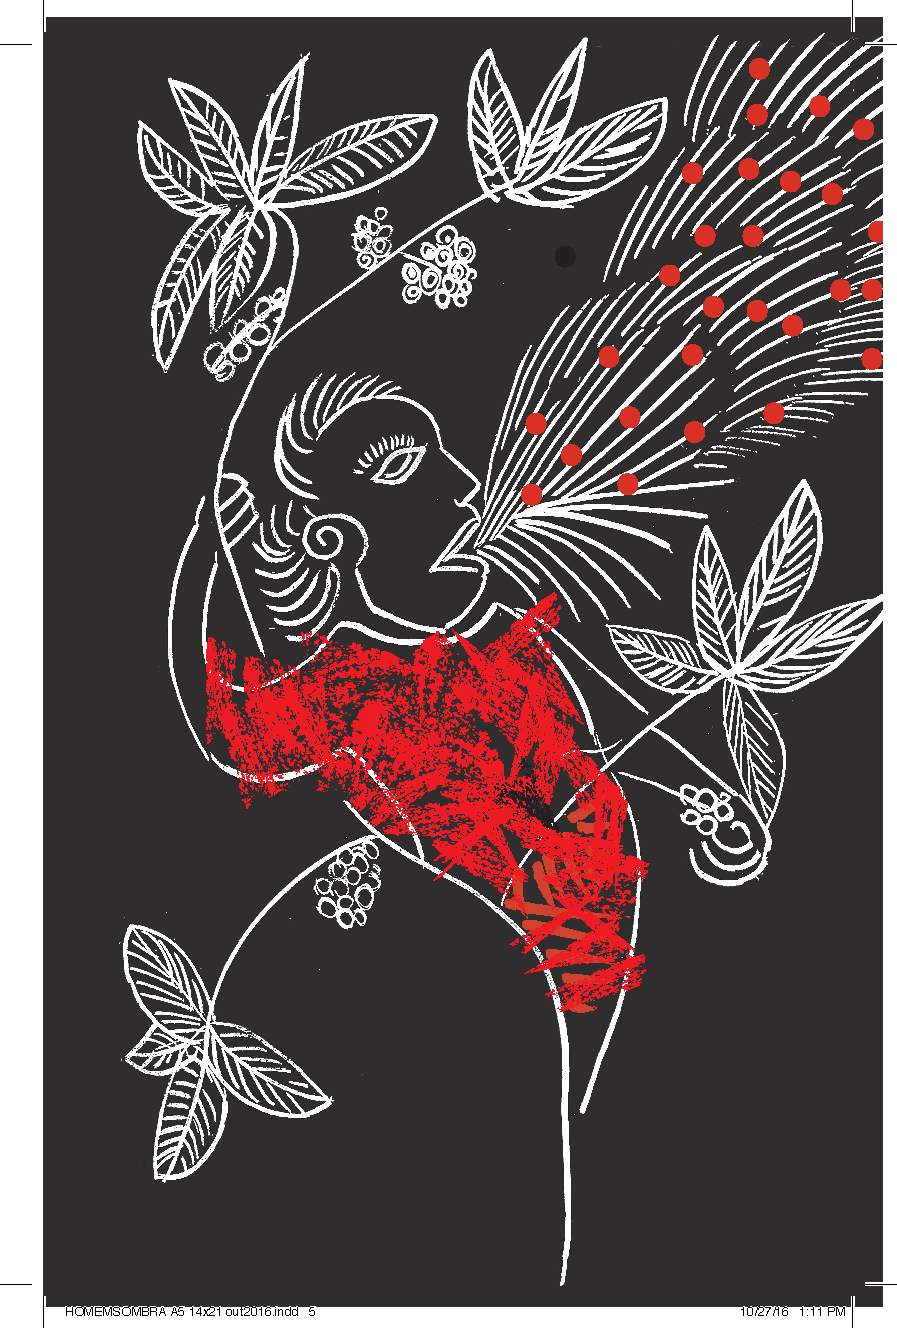
\includegraphics[width=153mm]{./imgs/img1.pdf}
\end{textblock*}

\chapter*{}

\mbox{}\vspace*{\fill}

\letra{E}{ncantado} com a música,
um homem hup aproximou-se,
sentou-se ao pé da
árvore e ficou escutando as
canções do homem-sombra. O
homem hup estava sentado,
pescando no igarapé
enquanto ouvia a música.

\vspace{2em}

\letra{P}{ɨ̗g} tëgan tɨh yam mɨ’ mah,
hup tɨh mɨ’ wɨ’ pemeh, tú.
Dë̖h máh hõ̖p käk pemep ɨhɨh.

\vspace*{\fill}

\pagebreak

\begin{textblock*}{8in}(0pt,0pt)%
\vspace*{-2.8cm}
\hspace*{-3.2cm}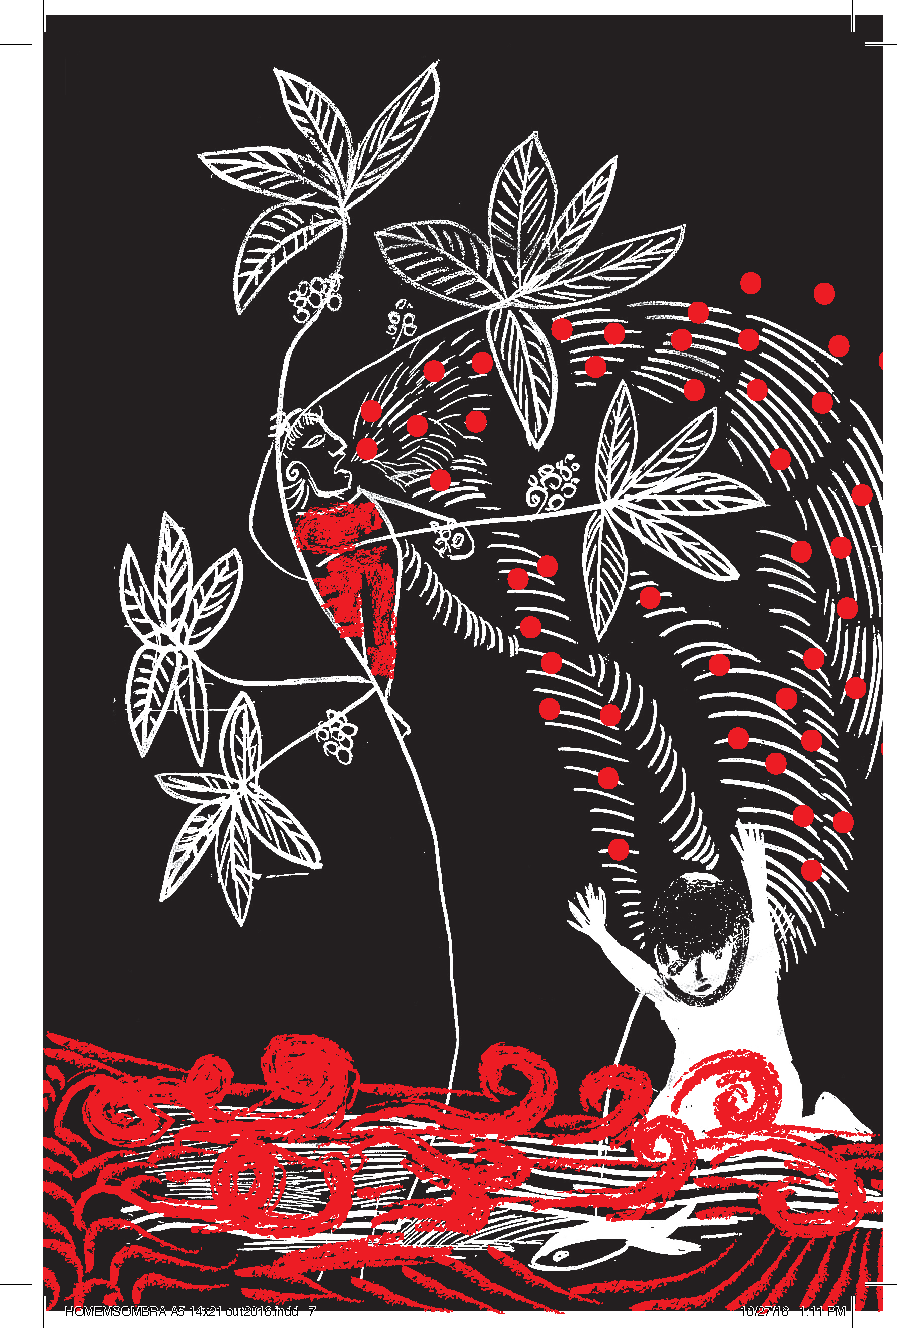
\includegraphics[width=153mm]{./imgs/img2.pdf}
\end{textblock*}

\chapter*{}

\mbox{}\vspace*{\fill}

\letra{D}{izem} que o Way Naku ficou
cantando e colhendo cucura
por muito tempo. O homem-sombra
ia de galho em galho
cantando e pegando os cachos
da fruta. Muitos dos cantos
que nós, Hupd’äh, cantamos nas
festas foram cantados pelo Way
Naku: o ``Canto do cutia'', o ``Canto
grande'', o ``Canto do Umarí'', o
``Canto da gente-sombra''.

\vspace{2em}

\letra{B}{ɨ̗ g!} mah tih yamah. Sã̗p nowot
pɨd, sã̗p nowot pɨd, pɨ̗g tëgët
tɨh noh k’ët kötöh, yamap ɨhɨh,
batɨ̗b’ih. \textit{Mèt Yam}, \textit{Yam Pög}, \textit{Pej
D’áp Yam}, \textit{Batɨ̗b’ Yam}, yám nihũ̗’
mah tɨ̗ h yamah!

\vspace*{\fill}

\pagebreak

\begin{textblock*}{8in}(0pt,0pt)%
\vspace*{-2.8cm}
\hspace*{-3.2cm}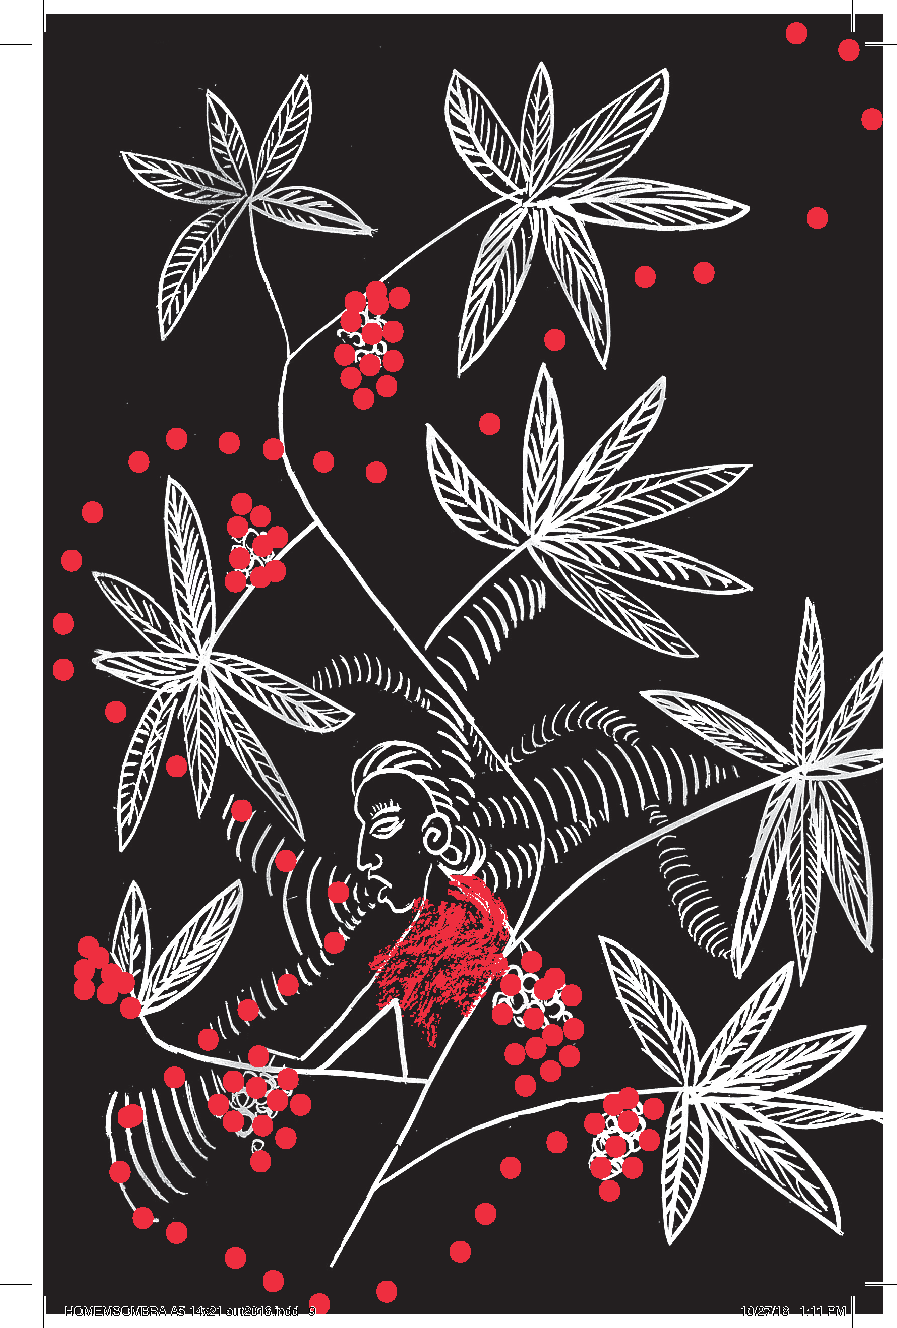
\includegraphics[width=153mm]{./imgs/img3.pdf}
\end{textblock*}

\chapter*{}

\mbox{}\vspace*{\fill}

\letra{O}{} homem hup ficou
lá a noite toda e,
depois, o outro dia
inteiro. Escutou e
prendeu os cantos
do homem-sombra.

\vspace{2em}

\letra{H}{iwag} yɨ’ɨy mah,
d’ú’ tɨh yam d’ö’öp\ldots{}

\vspace*{\fill}

\pagebreak

\begin{textblock*}{8in}(0pt,0pt)%
\vspace*{-2.8cm}
\hspace*{-3cm}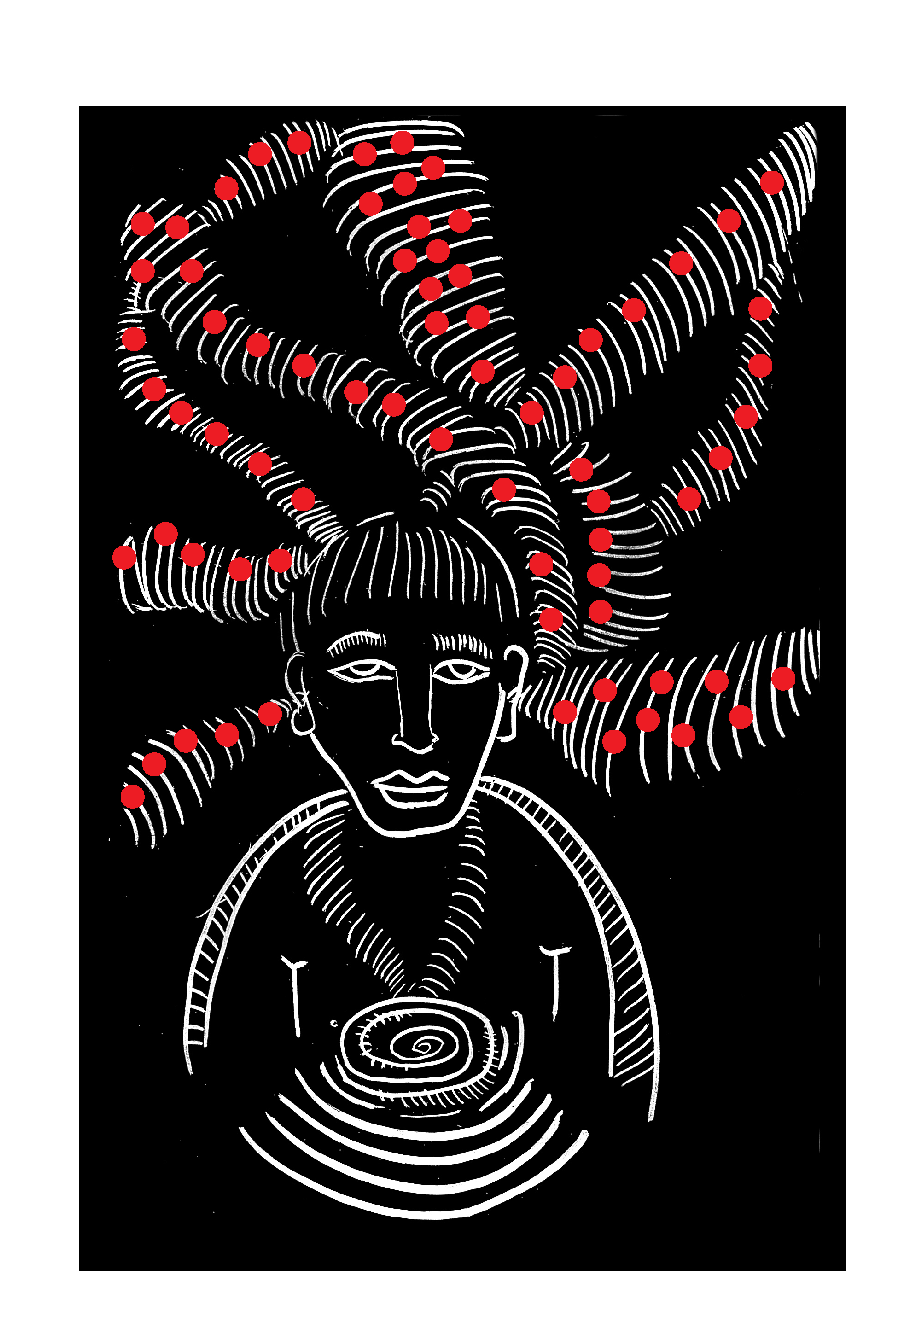
\includegraphics[width=148mm]{./imgs/img4.pdf}
\end{textblock*}

\chapter*{}

\mbox{}\vspace*{\fill}

\letra{Q}{uando} o sol
começou a nascer,
o homem hup bateu
com o terçado no
tronco da árvore
de cucura.

\vspace{2em}

\letra{H}{iwag} yɨ’ɨy, wag
hiyèt mah tɨh kɨt
hik’ëtayah, tɨh
të̖gët, pɨ̗ g tëgët.

\vspace*{\fill}

\pagebreak

\begin{textblock*}{8in}(0pt,0pt)%
\vspace*{-2.8cm}
\hspace*{-3.2cm}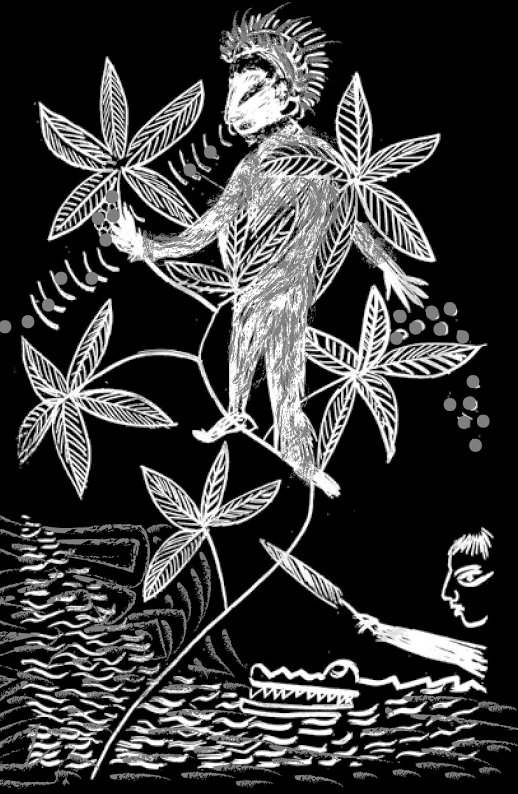
\includegraphics[width=153mm]{./imgs/img5.pdf}
\end{textblock*}

\chapter*{}

\mbox{}\vspace*{\fill}

\letra{T}{ac!} Foi o barulhão
que fez. Assustado,
o Way Naku caiu da
árvore. \textit{Puffff}!
Com medo, o homem
hup foi embora
correndo, bem
rápido! \textit{Vrummm}!

\vspace{2em}

\letra{T}{äk!} nomɨ’, yuway
mah tɨh kädhiayah.
\textit{Pë’}! Yuway mah
húp to’oh kädham
yɨ’ayah! \textit{Mmmm’}!

\vspace*{\fill}

\pagebreak

\begin{textblock*}{8in}(0pt,0pt)%
\vspace*{-2.8cm}
\hspace*{-3.2cm}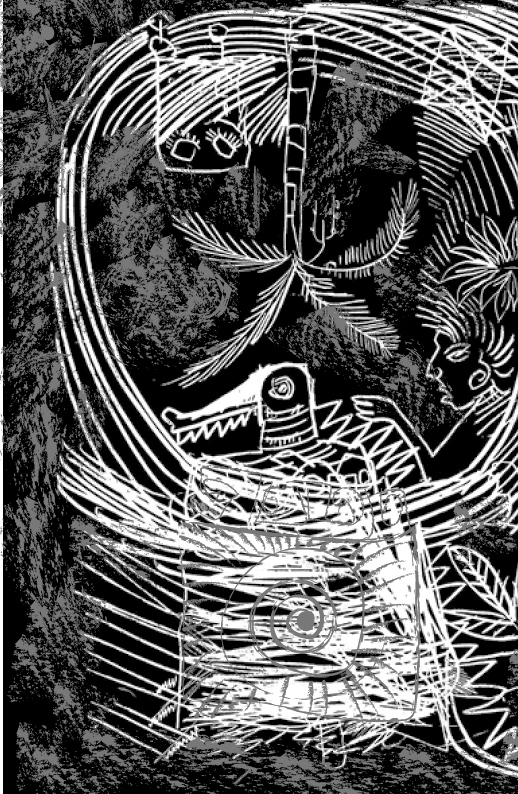
\includegraphics[width=153mm]{./imgs/img6.pdf}
\end{textblock*}

\chapter*{}

%\mbox{}\vspace*{\fill}

\letra{E}{ntão,} o Way Naku viu um
jacaré que estava deitado
na beira do rio. Pensou
que fosse o homem hup e
tentou pegá-lo. Fugindo,
o jacaré caiu na água,
\textit{tchibum}! O Way Naku,
que já estava na água,
foi atrás do jacaré. O
homem-sombra colocou a
mão na água para ver se
encontrava o jacaré.

\medskip

De repente, o jacaré deu uma\\
mordida no braço do\\
homem-sombra.

\vspace{2em}

\letra{Y}{ɨt} mah hàt yetníh. Yɨt
mah hàt noh tu’uh, \textit{tapuh}!
Yɨt mah tɨhɨt yɨ’ batɨ̗b’ noh
tu’ won kädd’öböh. Yɨt
mah hàtan tɨh d’ö’ yɨ’ɨh,
pëpë’ d’ö’ yɨ’ɨy.

\medskip

Yɨt mah tɨhan tɨh k’äç d’ö’\\
pög b’ayah, hàt b’ayah,\\
tɨnɨh mumùy súm,\\
batɨ̗b’anah.

\vspace*{\fill}

\pagebreak

\begin{textblock*}{8in}(0pt,0pt)%
\vspace*{-2.8cm}
\hspace*{-3.2cm}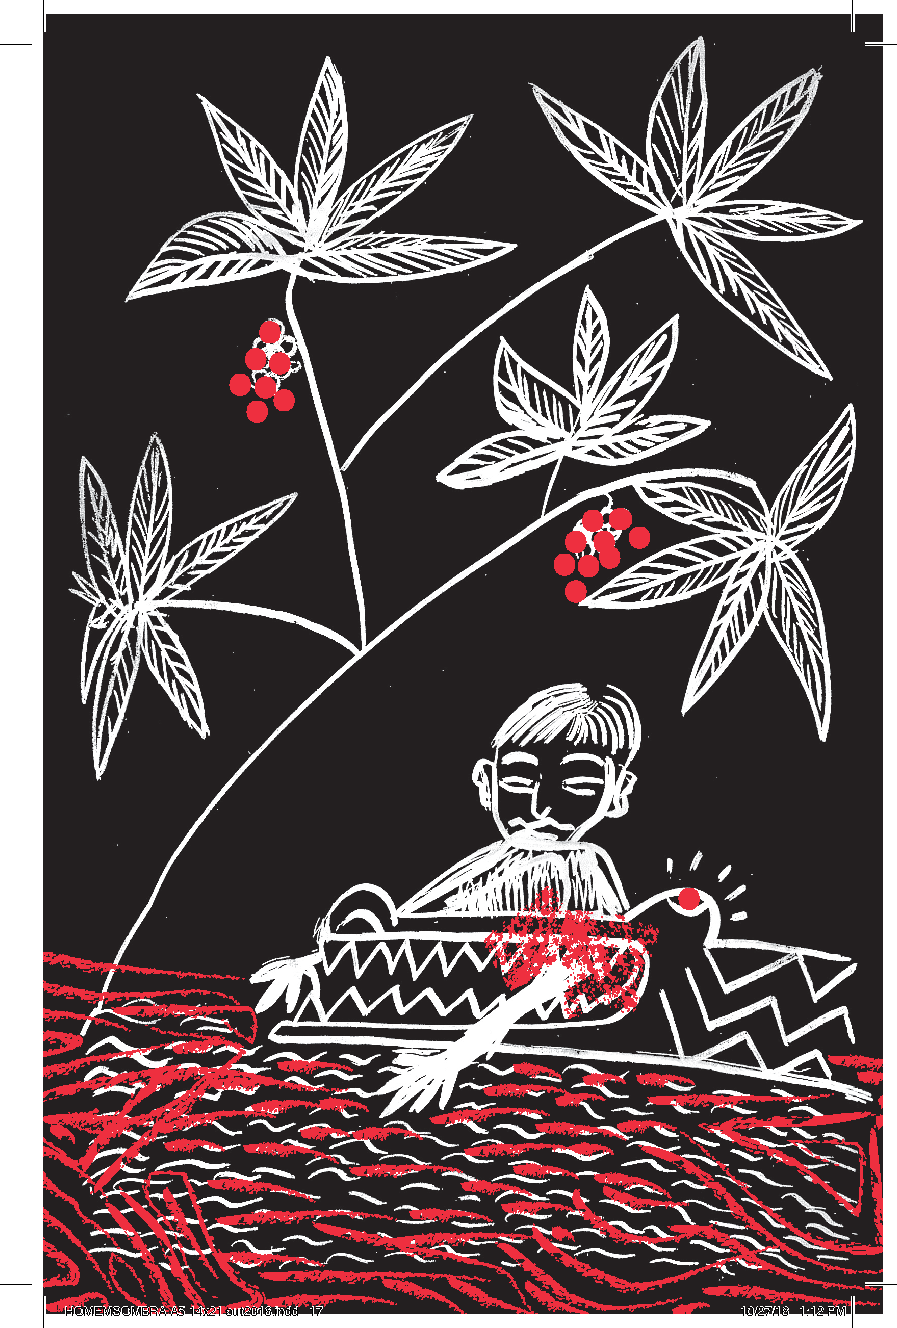
\includegraphics[width=153mm]{./imgs/img7.pdf}
\end{textblock*}

\chapter*{}

\mbox{}\vspace*{\fill}

\letra{E}{} foi assim que
o homem hup
conseguiu fugir e\\
voltar para casa.

\medskip

Esse foi o primeiro homem hup\\
que soube cantar os \textit{caapivaiá},\\
os cantos das festas.

\vspace{2em}

\letra{T}{ɨhɨp} húpup ham
yɨ’ay mah kah, yë
yɨ’ay mah.

\medskip

Yup ĩh mah yup, yám\\
d’ö’ hib’ahayah.

\vspace*{\fill}

\pagebreak

\begin{textblock*}{8in}(0pt,0pt)%
\vspace*{-2.8cm}
\hspace*{-3.2cm}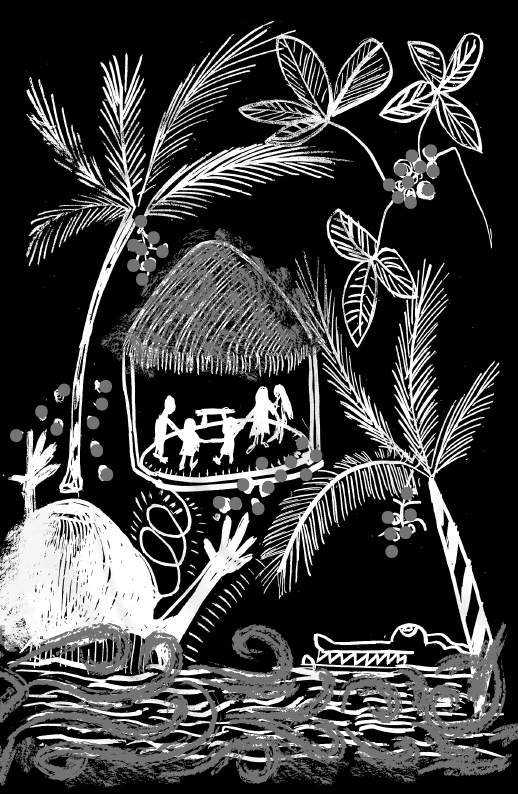
\includegraphics[width=153mm]{./imgs/img8.pdf}
\end{textblock*}

\chapter*{}

\mbox{}\vspace*{\fill}

\letra{E}{le} ouviu o homem-sombra cantar,
aprendeu bem e
começou a ensinar
para seus filhos,
irmãos, cunhados.
E até hoje todos
cantam e dançam os
\textit{caapivaiá} que animam\\
nossas festas.

\medskip

Foi isso o que ouvi de
meus avós.

\vspace{2em}

\letra{B}{atɨ̗b’} tɨh yamawan
wɨ’yö’ay mah, yup húp
yamayah. Yup hɨd yam
tëg n’ɨhayah. Húpd’äh
hɨd yam tëgayah.

\medskip

Ya’ap meh yɨ’ ãh wɨ’ɨh.

\vspace*{\fill}

\pagebreak

\begin{textblock*}{8in}(0pt,0pt)%
\vspace*{-2.8cm}
\hspace*{-3.2cm}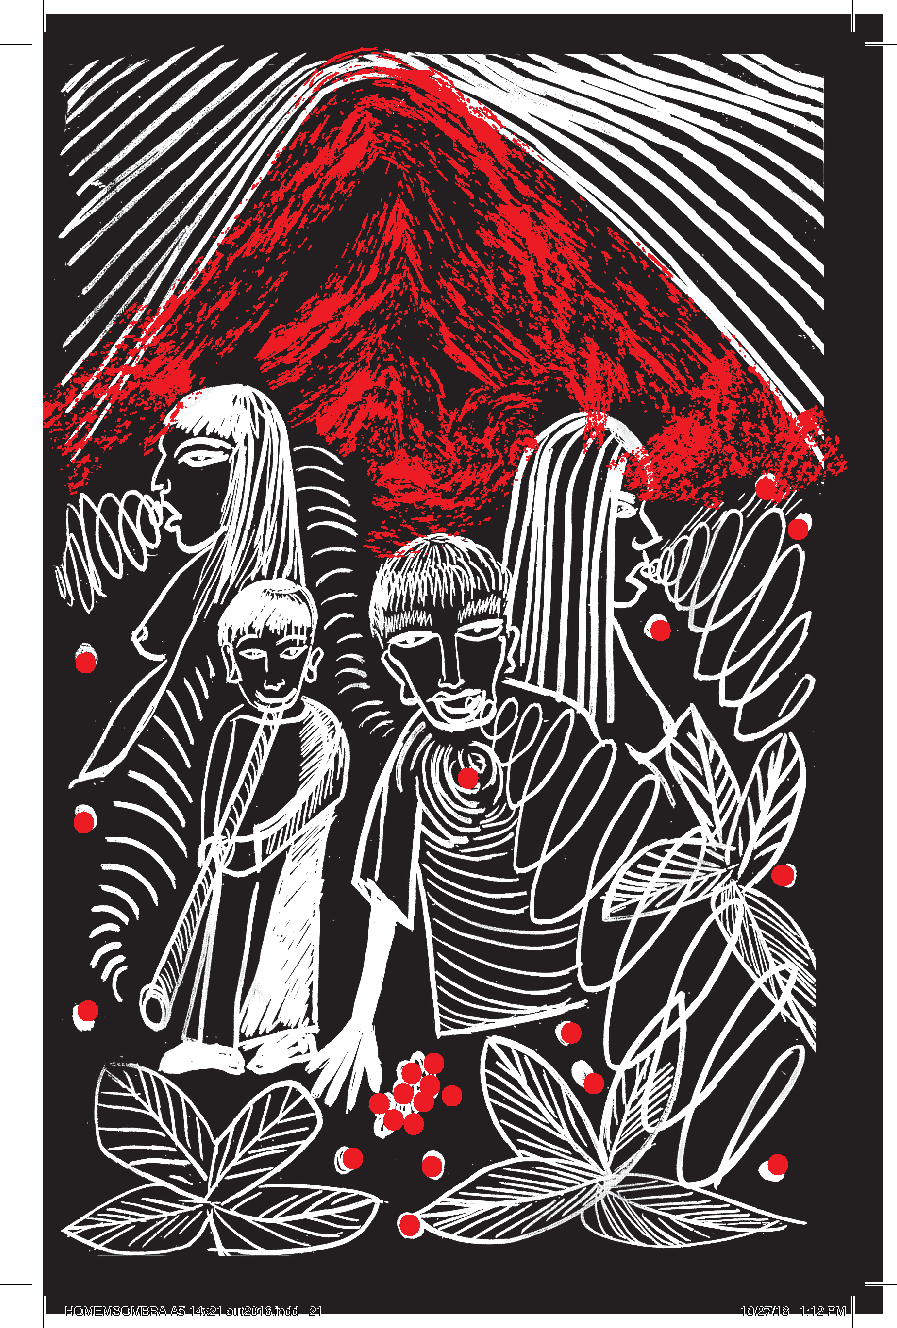
\includegraphics[width=153mm]{./imgs/img9.pdf}
\end{textblock*}

\endgroup

\addtocontents{toc}{\medskip}
\chapter{Glossário}

\paragraph{Caapivaiá} Cantos alegres de festa.

\paragraph{Cucura} \textls[15]{Fruta da floresta amazônica que nasce em cachos
como uma uvas. O nome científico é \textit{Pouroma Cecropiaefolia}.}

\paragraph{Cutia} \textls[-15]{Animal mamífero e roedor, pequeno, que vive na floresta. O nome
científico da cutia é \textit{Dasyprocta Fuliginosa}.}

\paragraph{Gente sombra} A gente sombra, homens e mulheres sombra, são
muito fortes e perigosos. Geralmente, causam doenças, podem matar
e comer a carne e o espírito das pessoas humanas. Muitos deles
são sábios e conhecem cantos, mitos e benzimentos. A cor de
sombra, de onde vem seu nome, é a cor de uma das roupas que essas gentes
usam para caçar e fazer mal às pessoas hup.

\paragraph{Homem sombra} Ser parecido com as pessoas
humanas, que vive na mata. Alguns, como Way Naku, vivem próximo a árvores frutíferas. Ele
é muito forte, sábio e poderoso. Ver \textit{Gente sombra}.

\paragraph{Terçado} Facão grande muito utilizado pelos Hupd’äh para cortar
galhos e árvores.

\paragraph{Umari} \textls[15]{Fruta da floresta amazônica de cor
amarela e de sabor um pouco amargo, muito apreciada pelos Hupd’äh.
Cresce numa árvore chamada umarizeiro, cujo o nome científico é \textit{Poraqueira Sp}.}



\pagebreak
\blankpage
\blankpage
\blankpage
%\blankAteven
\pagestyle{empty}
\begingroup
\fontsize{7}{8}\selectfont

{\large\textsc{coleção «hedra edições»}}

\begin{enumerate}
\setlength\parskip{4.2pt}
\setlength\itemsep{-1.4mm}
%\item \textit{Poemas da cabana montanhesa}, Saigy\=o
\item \textit{A arte da guerra}, Maquiavel
\item \textit{A conjuração de Catilina}, Salústio
\item \textit{A cruzada das crianças/ Vidas imaginárias}, Marcel Schwob
\item \textit{A filosofia na era trágica dos gregos}, Friedrich Nietzsche
\item \textit{A fábrica de robôs}, Karel Tchápek 
\item \textit{A história trágica do Doutor Fausto}, Christopher Marlowe
\item \textit{A metamorfose}, Franz Kafka
\item \textit{A monadologia e outros textos}, Gottfried Leibniz
\item \textit{A morte de Ivan Ilitch}, Lev Tolstói 
\item \textit{A velha Izerguil e outros contos}, Maksim Górki
\item \textit{A vida é sonho}, Calderón de la Barca
\item \textit{A volta do parafuso}, Henry James
\item \textit{A voz dos botequins e outros poemas}, Paul Verlaine 
\item \textit{A vênus das peles}, Leopold von Sacher{}-Masoch
\item \textit{A última folha e outros contos}, O.\,Henry
\item \textit{Americanismo e fordismo}, Antonio Gramsci
\item \textit{Anarquia pela educação}, Élisée Reclus 
\item \textit{Apologia de Galileu}, Tommaso Campanella 
\item \textit{Arcana C\oe lestia} e \textit{Apocalipsis revelata}, Emanuel Swedenborg
\item \textit{As bacantes}, Eurípides
\item \textit{Autobiografia de uma pulga}, [Stanislas de Rhodes]
\item \textit{Ação direta e outros escritos}, Voltairine de Cleyre
\item \textit{Balada dos enforcados e outros poemas}, François Villon
\item \textit{Carmilla, a vampira de Karnstein}, Sheridan Le Fanu
\item \textit{Carta sobre a tolerância}, John Locke
\item \textit{Contos clássicos de vampiro}, L.\,Byron, B.\,Stoker \& outros
\item \textit{Contos de amor, de loucura e de morte}, Horacio Quiroga
\item \textit{Contos indianos}, Stéphane Mallarmé
\item \textit{Cultura estética e liberdade}, Friedrich von Schiller
\item \textit{Cântico dos cânticos}, [Salomão]
\item \textit{Dao De Jing}, Lao Zi
\item \textit{Discursos ímpios}, Marquês de Sade
\item \textit{Dissertação sobre as paixões}, David Hume
\item \textit{Diário de um escritor (1873)}, Fiódor Dostoiévski
\item \textit{Diário parisiense e outros escritos}, Walter Benjamin
\item \textit{Diários de Adão e Eva}, Mark Twain
\item \textit{Don Juan}, Molière
\item \textit{Dos novos sistemas na arte}, Kazimir Maliévitch
\item \textit{Educação e sociologia}, Émile Durkheim
\item \textit{Édipo Rei}, Sófocles
\item \textit{Elogio da loucura}, Erasmo de Rotterdam
\item \textit{Émile e Sophie ou os solitários}, Jean-Jacques Rousseau 
\item \textit{Emília Galotti}, Gotthold Ephraim Lessing
\item \textit{Entre camponeses}, Errico Malatesta
\item \textit{Ernestine ou o nascimento do amor}, Stendhal
\item \textit{Escritos revolucionários}, Errico Malatesta
\item \textit{Escritos sobre arte}, Charles Baudelaire
\item \textit{Escritos sobre literatura}, Sigmund Freud
\item \textit{Eu acuso!}, Zola/\,\textit{O processo do capitão Dreyfus}, Rui Barbosa
\item \textit{Explosão: romance da etnologia}, Hubert Fichte
\item \textit{Fedro}, Platão
\item \textit{Feitiço de amor e outros contos}, Ludwig Tieck
\item \textit{Flossie, a Vênus de quinze anos}, [Swinburne]
\item \textit{Fábula de Polifemo e Galateia e outros poemas}, Góngora
\item \textit{Fé e saber}, Georg W.\,F.\,Hegel
\item \textit{Gente de Hemsö}, August Strindberg 
\item \textit{Hawthorne e seus musgos}, Melville
\item \textit{Hino a Afrodite e outros poemas}, Safo de Lesbos 
\item \textit{História da anarquia (vol.\,\textsc{ii})}, Max Nettlau
\item \textit{História da anarquia (vol.\,\textsc{i})}, Max Nettlau
\item \textit{Imitação de Cristo}, Tomás de Kempis
\item \textit{Incidentes da vida de uma escrava}, Harriet Jacobs
\item \textit{Inferno}, August Strindberg
\item \textit{Investigação sobre o entendimento humano}, David Hume
\item \textit{Jazz rural}, Mário de Andrade
\item \textit{Jerusalém}, William Blake
\item \textit{Joana d'Arc}, Jules Michelet
\item \textit{Lira gregra}, Giuliana Ragusa (org.)
\item \textit{Lisístrata}, Aristófanes 
\item \textit{Ludwig Feuerbach e o fim da filosofia clássica alemã}, Friederich Engels
\item \textit{Manifesto comunista}, Karl Marx e Friederich Engels
\item \textit{Memórias do subsolo}, Fiódor Dostoiévski
\item \textit{Metamorfoses}, Ovídio
\item \textit{Micromegas e outros contos}, Voltaire
\item \textit{Narrativa de William W.\,Brown, escravo fugitivo}, William Wells Brown
\item \textit{Nascidos na escravidão: depoimentos norte-americanos}, \textsc{wpa}
\item \textit{No coração das trevas}, Joseph Conrad
\item \textit{Noites egípcias e outros contos}, Aleksandr Púchkin
\item \textit{O casamento do Céu e do Inferno}, William Blake
\item \textit{O cego e outros contos}, \textsc{d.\,h}.\,Lawrence
\item \textit{O chamado de Cthulhu}, \textsc{h.\,p.}\,lovecraft
\item \textit{O contador de histórias e outros textos}, Walter Benjamin
\item \textit{O corno de si próprio e outros contos}, Marquês de Sade
\item \textit{O destino do erudito}, Johann Fichte
\item \textit{O estranho caso do dr.\,Jekyll e Mr. Hyde}, Robert Louis Stevenson
\item \textit{O fim do ciúme e outros contos}, Marcel Proust
\item \textit{O indivíduo, a sociedade e o Estado, e outros ensaios}, Emma Goldman
\item \textit{O ladrão honesto e outros contos}, Fiódor Dostoiévski
\item \textit{O livro de Monelle}, Marcel Schwob
\item \textit{O mundo ou tratado da luz}, René Descartes
\item \textit{O novo Epicuro: as delícias do sexo}, Edward Sellon
\item \textit{O pequeno Zacarias, chamado Cinábrio}, \textsc{e.\,t.\,a.}\,Hoffmann
\item \textit{O primeiro Hamlet}, William Shakespeare
\item \textit{O princípio anarquista e outros ensaios}, Piotr Kropotkin
\item \textit{O princípio do Estado e outros ensaios}, Mikhail Bakunin
\item \textit{O príncipe}, Maquiavel
\item \textit{O que eu vi, o que nós veremos}, Santos-Dumont
\item \textit{O retrato de Dorian Gray}, Oscar Wilde
\item \textit{O sobrinho de Rameau}, Diderot
\item \textit{Ode ao Vento Oeste e outros poemas}, \textsc{p.\,b.}\,Shelley
\item \textit{Ode sobre a melancolia e outros poemas}, John Keats
\item \textit{Odisseia}, Homero
\item \textit{Oliver Twist}, Charles Dickens
\item \textit{Origem do drama barroco}, Walter Benjamin
\item \textit{Os sofrimentos do jovem Werther}, Goethe
\item \textit{Os sovietes traídos pelos bolcheviques}, Rudolf Rocker
\item \textit{Para serem lidas à noite}, Ion Minulescu
\item \textit{Pensamento político de Maquiavel}, Johann Fichte
\item \textit{Pequeno-burgueses}, Maksim Górki
\item \textit{Pequenos poemas em prosa}, Charles Baudelaire
\item \textit{Perversão: a forma erótica do ódio}, Robert Stoller
\item \textit{Poemas}, Lord Byron
\item \textit{Poesia basca: das origens à Guerra Civil} 
\item \textit{Poesia catalã: das origens à Guerra Civil} 
\item \textit{Poesia espanhola: das origens à Guerra Civil} 
\item \textit{Poesia galega: das origens à Guerra Civil} 
\item \textit{Pr\ae terita}, John Ruskin
\item \textit{Primeiro livro dos Amores}, Ovídio
\item \textit{Rashômon e outros contos}, Ryūnosuke Akutagawa
\item \textit{Revolução e liberdade: cartas de 1845 a 1875}, Mikhail Bakunin
\item \textit{Robinson Crusoé}, Daniel Defoe
\item \textit{Romanceiro cigano}, Federico García Lorca
\item \textit{Sagas}, August Strindberg
\item \textit{Sobre a amizade e outros diálogos}, Jorge Luis Borges e Osvaldo Ferrari
\item \textit{Sobre a filosofia e outros diálogos}, Jorge Luis Borges e Osvaldo Ferrari
\item \textit{Sobre a filosofia e seu método (Parerga e paralipomena)} (v.\textsc{ii}, t.\textsc{i}), Arthur Schopenhauer 
\item \textit{Sobre a liberdade}, Stuart Mill
\item \textit{Sobre a utilidade e a desvantagem da histório para a vida}, Friedrich Nietzsche
\item \textit{Sobre a ética (Parerga e paralipomena)} (v.\textsc{ii}, t.\textsc{ii}), Arthur Schopenhauer 
\item \textit{Sobre anarquismo, sexo e casamento}, Emma Goldman
\item \textit{Sobre o riso e a loucura}, [Hipócrates]
\item \textit{Sobre os sonhos e outros diálogos}, Jorge Luis Borges e Osvaldo Ferrari
\item \textit{Sobre verdade e mentira}, Friedrich Nietzsche
\item \textit{Sonetos}, William Shakespeare
\item \textit{Sátiras, fábulas, aforismos e profecias}, Leonardo da Vinci
\item \textit{Teleny, ou o reverso da medalha}, Oscar Wilde
\item \textit{Teogonia}, Hesíodo
\item \textit{Trabalhos e dias}, Hesíodo
\item \textit{Triunfos}, Petrarca
\item \textit{Um anarquista e outros contos}, Joseph Conrad
\item \textit{Viagem aos Estados Unidos}, Alexis de Tocqueville
\item \textit{Viagem em volta do meu quarto}, Xavier de Maistre 
\item \textit{Viagem sentimental}, Laurence Sterne
\end{enumerate}

{\large\textsc{coleção «metabiblioteca»}}

\begin{enumerate}
\setlength\parskip{4.2pt}
\setlength\itemsep{-1.4mm}
\item \textit{A carteira de meu tio}, Joaquim Manuel de Macedo
\item \textit{A cidade e as serras}, Eça de Queirós
\item \textit{A escrava}, Maria Firmina dos Reis
\item \textit{A família Medeiros}, Júlia Lopes de Almeida 
\item \textit{A pele do lobo e outras peças}, Artur Azevedo
\item \textit{Auto da barca do Inferno}, Gil Vicente
\item \textit{Bom Crioulo}, Adolfo Caminha
\item \textit{Cartas a favor da escravidão}, José de Alencar
\item \textit{Contos e novelas}, Júlia Lopes de Almeida
\item \textit{Crime}, Luiz Gama
\item \textit{Democracia}, Luiz Gama
\item \textit{Direito}, Luiz Gama
\item \textit{Elixir do pajé: poemas de humor, sátira e escatologia}, Bernardo Guimarães
\item \textit{Eu}, Augusto dos Anjos
\item \textit{Farsa de Inês Pereira}, Gil Vicente
\item \textit{Helianto}, Orides Fontela
\item \textit{História da província Santa Cruz}, Gandavo
\item \textit{Iracema}, José de Alencar
\item \textit{Liberdade}, Luiz Gama
\item \textit{Mensagem}, Fernando Pessoa
\item \textit{Nós, os sul-americanos}, Flávio de Carvalho
\item \textit{O Ateneu}, Raul Pompeia
\item \textit{O cortiço}, Aluísio Azevedo
\item \textit{O desertor}, Silva Alvarenga
\item \textit{Oração aos moços}, Rui Barbosa
\item \textit{Pai contra mãe e outros contos}, Machado de Assis
\item \textit{Poemas completos de Alberto Caeiro}, Fernando Pessoa
\item \textit{Teatro de êxtase}, Fernando Pessoa
\item \textit{Transposição}, Orides Fontela
\item \textit{Tratado descritivo do Brasil em 1587}, Gabriel Soares de Sousa
\item \textit{Tratados da terra e gente do Brasil}, Fernão Cardim 
\item \textit{Utopia Brasil}, Darcy Ribeiro
\item \textit{Índice das coisas mais notáveis}, Antônio Vieira
\end{enumerate}

\medskip
{\large\textsc{coleção «que horas são?»}}

\begin{enumerate}
\setlength\parskip{4.2pt}
\setlength\itemsep{-1.4mm}
\item \textit{8/1: A rebelião dos manés}, Pedro Fiori Arantes, Fernando Frias e Maria Luiza Meneses
\item \textit{A linguagem fascista}, Carlos Piovezani \& Emilio Gentile
\item \textit{A sociedade de controle}, J.\,Souza; R.\,Avelino; S.\,Amadeu (orgs.)
\item \textit{Ativismo digital hoje}, R.\,Segurado; C.\,Penteado; S.\,Amadeu (orgs.)
\item \textit{Crédito à morte}, Anselm Jappe
\item \textit{Descobrindo o Islã no Brasil}, Karla Lima
\item \textit{Desinformação e democracia}, Rosemary Segurado
\item \textit{Dilma Rousseff e o ódio político}, Tales Ab'Sáber
\item \textit{Labirintos do fascismo} (v.\textsc{iii}), João Bernardo
\item \textit{Labirintos do fascismo} (v.\textsc{ii}), João Bernardo
\item \textit{Labirintos do fascismo} (v.\textsc{iv}), João Bernardo
\item \textit{Labirintos do fascismo} (v.\textsc{i}), João Bernardo
\item \textit{Labirintos do fascismo} (v.\textsc{vi}), João Bernardo
\item \textit{Labirintos do fascismo} (v.\textsc{v}), João Bernardo
\item \textit{Lugar de negro, lugar de branco?}, Douglas Rodrigues Barros
\item \textit{Lulismo, carisma pop e cultura anticrítica}, Tales Ab'Sáber
\item \textit{Machismo, racismo, capitalismo identitário}, Pablo Polese
\item \textit{Michel Temer e o fascismo comum}, Tales Ab'Sáber
\item \textit{O quarto poder: uma outra história}, Paulo Henrique Amorim
\item \textit{Universidade, cidade e cidadania}, Franklin Leopoldo e Silva
\end{enumerate}

\medskip
{\large\textsc{coleção «mundo indígena»}}

\begin{enumerate}
\setlength\parskip{4.2pt}
\setlength\itemsep{-1.4mm}
\item \textit{A folha divina}, Timóteo Verá Tupã Popygua
\item \textit{A mulher que virou tatu}, Eliane Camargo
\item \textit{A terra uma só}, Timóteo Verá Tupã Popygua
\item \textit{A árvore dos cantos}, Pajés Parahiteri
\item \textit{Cantos dos animais primordiais}, Ava Ñomoandyja Atanásio Teixeira
\item \textit{Crônicas de caça e criação}, Uirá Garcia
\item \textit{Círculos de coca e fumaça}, Danilo Paiva Ramos
\item \textit{Folhas divinas}, Timóteo Verá Tupã Popygua
\item \textit{Nas redes guarani}, Valéria Macedo \& Dominique Tilkin-Gallois
\item \textit{Não havia mais homens}, Luciana Storto
\item \textit{O surgimento da noite}, Pajés Parahiteri
\item \textit{O surgimento dos pássaros}, Pajés Parahiteri
\item \textit{Os Aruaques}, Max Schmidt
\item \textit{Os cantos do homem-sombra}, Patience Epps e Danilo Paiva Ramos
\item \textit{Os comedores de terra}, Pajés Parahiteri
\item \textit{Xamanismos ameríndios}, A.\,Barcelos Neto, L.\,Pérez Gil \& D.\,Paiva Ramos
\end{enumerate}

\medskip
{\large\textsc{coleção «ecopolítica»}}

\begin{enumerate}
\setlength\parskip{4.2pt}
\setlength\itemsep{-1.4mm}
\item \textit{Anarquistas na América do Sul}, E.\,Passetti, S.\,Gallo; A.\,Augusto  (orgs.)
\item \textit{Ecopolítica}, E.\,Passetti; A.\,Augusto; B.\,Carneiro; S.\,Oliveira, T.\,Rodrigues  (orgs.)
\item \textit{Pandemia e anarquia}, E.\,Passetti; J.\,da Mata; J.\,Ferreira  (orgs.)
\end{enumerate}

% \medskip
% {\large\textsc{coleção <<anarc>>}}

% \begin{enumerate}
% \setlength\parskip{4.2pt}
% \setlength\itemsep{-1.4mm}
% \item \textit{Anarquia pela educação}, Élisée Reclus 
% \item \textit{Ação direta e outros escritos}, Voltairine de Cleyre
% \item \textit{Entre camponeses}, Errico Malatesta
% \item \textit{Escritos revolucionários}, Errico Malatesta
% \item \textit{História da anarquia (vol.\,\textsc{ii})}, Max Nettlau
% \item \textit{História da anarquia (vol.\,\textsc{i})}, Max Nettlau
% \item \textit{O indivíduo, a sociedade e o Estado, e outros ensaios}, Emma Goldman
% \item \textit{O princípio anarquista e outros ensaios}, Piotr Kropotkin
% \item \textit{O princípio do Estado e outros ensaios}, Mikhail Bakunin
% \item \textit{Os sovietes traídos pelos bolcheviques}, Rudolf Rocker
% \item \textit{Revolução e liberdade: cartas de 1845 a 1875}, Mikhail Bakunin
% \item \textit{Sobre anarquismo, sexo e casamento}, Emma Goldman
% \end{enumerate}

% \medskip
% {\large\textsc{coleção <<narrativas da escravidão>>}}

% \begin{enumerate}
% \setlength\parskip{4.2pt}
% \setlength\itemsep{-1.4mm}
% \item \textit{Incidentes da vida de uma escrava}, Harriet Jacobs
% \item \textit{Narrativa de William W.\,Brown, escravo fugitivo}, William Wells Brown
% \item \textit{Nascidos na escravidão: depoimentos norte-americanos}, \textsc{wpa}
% \end{enumerate}

\pagebreak
\pagebreak

%\ifodd\thepage\blankpage\fi

\parindent=0pt
\footnotesize\thispagestyle{empty}

% \noindent\textbf{Dados Internacionais de Catalogação na Publicação -- CIP}\\
% \noindent\textbf{(Câmara Brasileira do Livro, SP, Brasil)}\\

% \dotfill\\

% \hspace{20pt}ISBN 978-65-86238-31-0 (Livro do Estudante)

% \hspace{20pt}ISBN 978-65-86238-30-3 (Manual do Professor)\\[6pt]

% \hspace{20pt}\parbox{190pt}{1. Crônicas Brasileira. 2. Contos Brasileiro. 3. Rosa, Alexandre. I. Título.}\\[6pt]

% \hspace{188pt}\textsc{cdd}-B869.8

% \dotfill

% \noindent{}Elaborado por Regina Célia Paiva da Silva CRB -- 1051\\

\mbox{}\vfill
\begin{center}
		\begin{minipage}{.7\textwidth}\tiny\noindent{}
		\centering\tiny
		Adverte-se aos curiosos que se imprimiu este livro na data de \today, em papel pólen bold, composto em tipologia Libertine e Formular, em 11 pontos, com diversos sofwares livres,
		dentre eles Lua\LaTeX e git.\\ 
		\ifdef{\RevisionInfo{}}{\par(v.\,\RevisionInfo)}{}\medskip\\\
		\adforn{64}
		\end{minipage}
\end{center}

%\input{SOL}
%\input{GOKYP}
%\input{LUA}
%\input{OTI}
%\input{RITUAL}
%\input{OSIIP}
%\input{ENCONTRO1}
%\input{ENCONTRO2}
%\input{BIOS}
